\documentclass[a4paper]{article} 
\usepackage{graphics}
\usepackage{graphicx}
\usepackage{color}
\usepackage{hyperref}
\usepackage{amsmath}
\usepackage{enumerate}
\usepackage[a4paper, total={14.5cm, 24cm}]{geometry}
\usepackage{multicol}


%\pagestyle{fancy}
%\fancyhf{}
%\fancyhead[LE, RO]{Jug\u anaru C\u alin}
%\fancyhead[RE, LO]{ Probleme de t\u aietur\u a }

\title{\Huge \bfseries Tema 2 \\[1.5cm]  \Large la disciplina \textit{Bazele electrotehnicii} \\[10cm]} \par

\author{\\[1cm] \Large C\u alin Jug\u anaru, 314CA 
	\\[1.8cm] Universitatea POLITEHNICA din Bucure\c sti 
	\\[0.4cm] Facultatea de Automatic\u a \c si Calculatoare
	\\[2cm] calin\_vlad.juganaru@stud.acs.upb.ro \\}

\begin{document}
\maketitle
\pagebreak
\renewcommand{\contentsname}{ \huge \bfseries Cuprins}
\renewcommand{\refname}{Bibliografie}

\tableofcontents
\newpage

% ----------------------------------------------------------------------------------------------------------------------------------------------------------------
% --------------------------------------------------------------------------- 1 ----------------------------------------------------------------------------------

\title{\huge \center Circuite electrice de curent alternativ \c si tranzitoriu} \\
\maketitle

\begin{section}{Rezolvarea circuitelor de curent alternativ}
\begin{subsection}{Trecerea din real \^ in complex\\}

	\^ In cadrul circuitului generat pentru prima tem\u a am ad\u augat bobina $ L, $ \^ in serie cu rezistorul $ R_3, $ \c si condensatorul $ C, $ \^ in paralel cu rezistorul $ R_2 $. Pentru urm\u atorul pas vom \^ inlocui toate sursele independente de curent \c si tensiune cu surse sinusoidale, apoi vom trece toate m\u arimile din real \^ in complex: 

\begin{center} 
	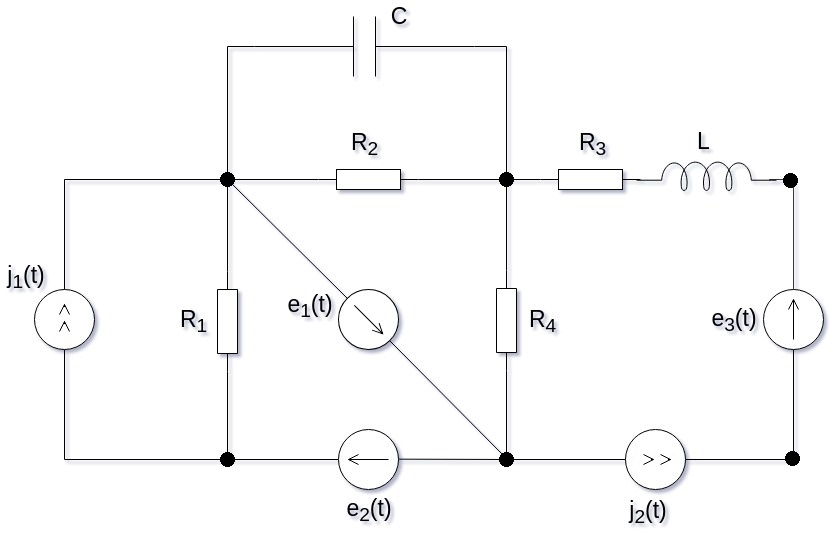
\includegraphics[width=13cm, height=8cm]{circuitsin.jpg} \\ 
	Noul circuit, cu surse sinusoidale \\[1.425cm]
	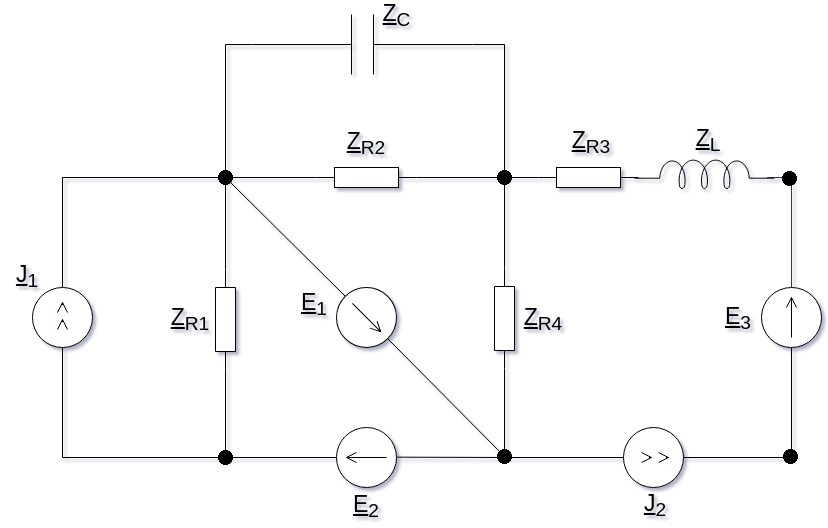
\includegraphics[width=13cm, height=8cm]{circuitC.jpg} \\
	Reprezentarea \^ in complex a circuitului  \\[1cm] 
\end{center}

% -------------------------------------------------------------------------- a) ----------------------------------------------------------------------------------

	Dup\u a ad\u augarea noilor elemente de circuit, perechea de grafuri orientate $(G_I, G_U)$, corespunz\u atoare grafului de curen\c ti, respectiv de tensiuni ale circuitului electric ales trebuie modificate prin ad\u augarea unei noi laturi, aceea pe care se afl\u a condensatorul, \c si, implicit, a unui nou curent \c si a unei noi tensiuni corespunz\u atoare acelei laturi (acestea vor fi $ I_{10} $, respectiv $ U_{10} $).
	De asemenea, prin ad\u augarea unei noi laturi pe graf, num\u arul total de laturi \c si bucle va cre\c ste cu 1. Deci \large $$ (N, L, B) = (6, 10, 5). $$ \\ \normalsize
\par

\begin{center} 
	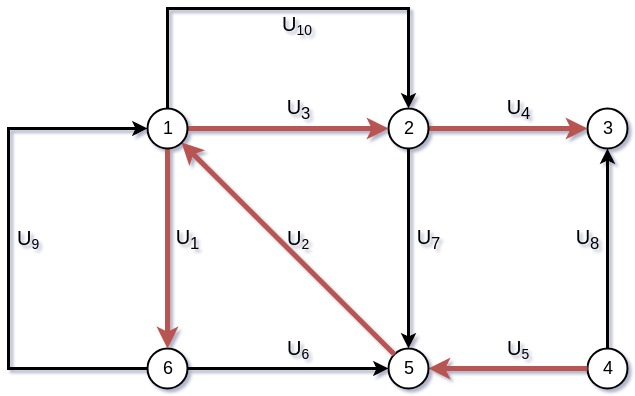
\includegraphics[width=13cm, height=8cm]{grafU.jpg} \\ 
	Graful de tensiuni, av\^ and arborele eviden\c tiat cu ro\c su \\[1.7cm]
	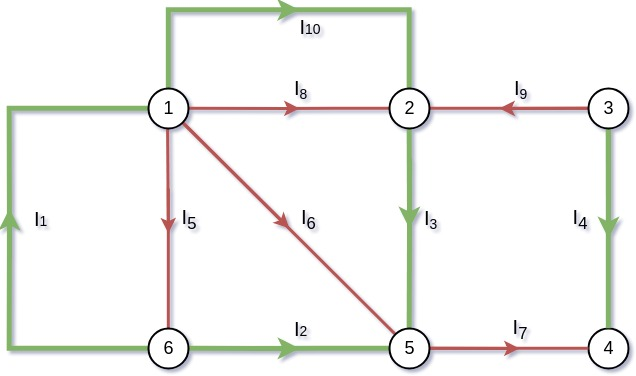
\includegraphics[width=13cm, height=8cm]{grafI.jpg} \\
	Graful de curen\c ti, av\^ and coarborele eviden\c tiat cu verde  \\[1cm] 
\end{center}

	Proced\^ and ca la prima tem\u a, pentru a afla valorile tuturor m\u arimilor elementelor de circuit, tensiunilor \c si curen\c tilor de pe laturi, putem folosi metoda arborelui: alegem un arbore maximal de acoperire pe graf, apoi fix\u am tensiunile de pe ramurile arborelui \c si curen\c tii de pe coardele coarborelui. Dac\u a aceste valori alese ini\c tial sunt numere \^ intregi, aplic\^ and teoremele I \c si II ale lui Kirchhoff, toate celelalte valori vor fi, de asemenea, \^ intregi. 

Astfel, tensiunile alese ini\c tial pe ramurile arborelui \c si intensit\u a\c tile alese pe coardele coarborelui sunt:

\begin{multicols}{2}
\begin{large}
	\begin{itemize}
		\item $ U_1 = 2 $ V
		\item $ U_2 = 5 $ V
		\item $ U_3 = 3 $ V
		\item $ U_4 = 2 $ V
		\item $ U_5 = 1 $ V

		\item $ I_1 = 6 $ A
		\item $ I_2 = 4 $ A
		\item $ I_3 = 3 $ A
		\item $ I_4 = -2 $ A
		\item $ I_{10} = 1 $ A

	\end{itemize} \par
\end{large}
\end{multicols}

De aici, putem aplica foarte simplu teoremele I \c si II ale lui Kirchhoff pentru aflarea tuturor celorlalte tensiuni \c si intensit\u a\c ti. Astfel, 

\begin{multicols}{2}
\begin{large}
	\begin{itemize}
		\item $ [1]: U_9 = -U_1 $
		\item $ [2]: U_6 = -U_1 - U_2 $
		\item $ [3]: U_7 = -U_2 - U_3 $
		\item $ [4]: U_8 = U_4 + U_5 - U_7 $
		\item $ [5]: U_{10} = U_3 $
		
		\item $ (2): I_8 = I_3 - I_9 $
		\item $ (3): I_9 = - I_4 $
		\item $ (4): I_7 = - I_4 $
		\item $ (5): I_6 = I_7 - I_2 - I_3 $
	\end{itemize} \par
\end{large}
\end{multicols}

unde $ (n) $ este nodul, iar $ [b] $ este bucla pe care au fost aplicate teoremele lui Kirchhoff. \\[0.5cm]
Din aceste rela\c tii rezult\u a valorile: 

\begin{multicols}{2}
\begin{large}
	\begin{itemize}
		\item $ U_6 = -7 $ V
		\item $ U_7 = -8 $ V
		\item $ U_8 = 11 $ V
		\item $ U_9 = -2 $ V
		\item $ U_{10} = 3 $ V

		\item $ I_6 = -5 $ A
		\item $ I_7 = 2 $ A
		\item $ I_8 = 1 $ A
		\item $ I_9 = 2 $ A
	\end{itemize} \par
\end{large}
\end{multicols}

	Putem observa c\u a unele dintre aceste valori, alese ini\c tial sau calculate mai sus, reprezint\u a tensiunile sau curen\c tii electromotori debita\c ti de sursele ideale din circuit, mai exact:

\begin{multicols}{2}
\begin{large}
	\begin{itemize}
		\item $ E_1 = U_2 = -5$ V
		\item $ E_2 = U_6 = -7$ V
		\item $ E_3 = -U_8 = -11$  V
		
		\item $ J_1 = I_1 = 6 $ A
		\item $ J_2 = I_7 = 2 $ A \\
	\end{itemize} \par
\end{large}
\end{multicols}

	Tot din aceste valori de tensiuni \c si intensit\u a\c ti calculate, putem deduce \c si rezisten\c tele de pe laturi:

\begin{multicols}{2}
\begin{large}
	\begin{itemize}
		\item $ R_1 = \frac{U_1}{I_5} =  \frac{1}{5}$ $ \Omega $
		\item $ R_2 = \frac{U_3}{I_8} = 3$ $ \Omega $
		\item $ R_3 = \frac{U_4}{I_9} = 1$ $ \Omega $
		\item $ R_4 = \frac{U_7}{I_3} = - \frac{8}{3} $ $ \Omega $ 
	\end{itemize} \par
\end{large}
\end{multicols}

	 Cum $ R_2 = 3 $ $ \Omega $ \c si $ R_3 = 1 $ $ \Omega $, rezult\u a c\u a $ L = \frac{100}{\pi} $ $ mH $, iar $ C = \frac{300}{\pi} $ $ \mu F $.
	\^ In continuare, vom folosi valorile rezisten\c telor calculate, ale bobinei \c si condensatorului ad\u augate ulterior, precum \c si expresiile sinusoidale ale surselor pentru a calcula toate tensiunile \c si intensit\u a\c tile. \\  \par

	Consider\^ and tesiunile \c si curen\c tii electromotori de mai sus ca valori efective \c si aleg\^ and diferite valori pentru fazele ini\c tiale, ob\c tinem func\c tiile sinusoidale:

\begin{multicols}{2}
\begin{large}
	\begin{itemize}
		\item $ e_1(t) = E_1 \sqrt2 \sin{(\omega t)} $
		\item $ e_2(t) = E_2 \sqrt2 \sin{(\omega t - \frac{\pi}{2})} $
		\item $ e_3(t) = E_3 \sqrt2 \sin{(\omega t + \frac{\pi}{2})} $
		
		\item $ j_1(t) = J_1 \sqrt2 \sin{(\omega t - \frac{\pi}{4})} $
		\item $ j_2(t) = J_2 \sqrt2 \sin{(\omega t + \frac{\pi}{4})} $ \\
	\end{itemize} \par
\end{large}
\end{multicols}

	Cum frecven\c ta $ f $ este impus\u a din enun\c t ($ 50 $ $ Hz $), iar pulsa\c tia  este $ 2\pi f$, rezult\u a c\u a $ \omega = 100\pi $. \^ Inlocuind pulsa\c tia \c si valorile efective \^ in rela\c tiile de mai sus, ob\c tinem sistemul: 

\begin{multicols}{2}
\begin{large}
	\begin{itemize}
		\item $ e_1(t) = -5 \sqrt2 \sin{(100\pi t)} $
		\item $ e_2(t) = -7 \sqrt2 \sin{(100\pi t - \frac{\pi}{2})} $
		\item $ e_3(t) = -11 \sqrt2 \sin{(100\pi t + \frac{\pi}{2})} $
		
		\item $ j_1(t) = 6 \sqrt2 \sin{(100\pi t - \frac{\pi}{4})} $
		\item $ j_2(t) = 2 \sqrt2 \sin{(100\pi t + \frac{\pi}{4})} $ \\
	\end{itemize} \par
\end{large}
\end{multicols}

Folosind formulele \large 

 \begin{large} \[ \left\{ \begin{array}{ll}
$$ x(t) = X\sqrt2 \cdot sin(\omega t + \phi) $$ \\
$$ \underline{X} = X e^{j\phi}  = Xcos(\phi) + jXsin(\phi) $$
\end{array} \right. \] \end{large}
 \normalsize \c si \^ inlocuind \^ in rela\c tiile de mai sus pentru valorile noastre, ob\c tinem:

\begin{multicols}{2}
\begin{large}
	\begin{itemize}
		\item $ \underline{E_1} = -5cos(0) -5j \cdot sin(0) $
		\item $ \underline{E_2} = -7cos(-\frac{\pi}{2}) -7j \cdot sin(-\frac{\pi}{2}) $
		\item $ \underline{E_3} = -11cos(\frac{\pi}{2}) -11j \cdot sin(\frac{\pi}{2}) $
		
		\item $ \underline{J_1} = 6cos(-\frac{\pi}{4}) + 6j \cdot sin(-\frac{\pi}{4}) $
		\item $ \underline{J_2} = 2cos(\frac{\pi}{4}) + 2j \cdot sin(\frac{\pi}{4}) $ \\
	\end{itemize} \par
\end{large}
\end{multicols}

	\^ In final, \^ inlocuind \c si cu valorile sinusurilor \c si cosinusurilor, rezult\u a valorile complexe:

\begin{multicols}{2}
\begin{large}
	\begin{itemize}
		\item $ \underline{E_1} = -5 $
		\item $ \underline{E_2} = 7j $
		\item $ \underline{E_3} = -11j $
		
		\item $ \underline{J_1} = 3\sqrt2 -3j \sqrt2 $
		\item $ \underline{J_2} = \sqrt2 + j \sqrt2 $ \\
	\end{itemize} \par
\end{large}
\end{multicols}

	Rezisten\c tele trecute \^ in complex \^ i\c si p\u astreaz\u a valoarea, schimb\^ andu-se doar nota\c tia \c si denumirea (din rezisten\c ta $ R $ \^ in impedan\c ta complex\u a $ \underline{Z} $). Pentru bobin\u a \c si condensator, valorile impedan\c telor complexe vor fi: \\

\begin{large} \[ \left\{ \begin{array}{ll}
		\underline{Z}_L = j \omega L = \frac{100 j \cdot 100 \pi}{\pi} = 10^4j \\[0.1cm]
		\underline{Z}_C = -\frac{j}{\omega C} = -\frac{j \pi}{300 \cdot 100 \pi} = -\frac{10^{-4}}{3} j \\
\end{array} \right. \] \end{large}

\end{subsection}
\pagebreak

% -------------------------------------------------------------------------- b) ----------------------------------------------------------------------------------
\begin{subsection}{Rezolvarea sistemului de ecua\c tii \\}

	Pentru a afla rela\c tiile dintre necunoscute \c si rezolva sistemul de ecua\c tii, rezult\^ and valorile tuturor curen\c tilor \c si tensiunilor din circuit, putem aplica metoda ecua\c tiilor lui Kirchhoff. \^ In plus fa\c t\u a de prima tem\u a, la sistemul de ecua\c tii voim ad\u auga \^ inc\u a un curent \c si o tensiune, corespunz\u atoare noii laturi:
 
\begin{itemize}
	\item Aplic\u am teorema I a lui Kirchhoff pentru $ N - 1 $ noduri:
	
 	\begin{large} \[ \left\{ \begin{array}{ll}
		(1): \underline{I}_1 =  \underline{I}_5 + \underline{I}_6 + \underline{I}_8 + \underline{I}_{10} \\
		(2): \underline{I}_8 + \underline{I}_9  + \underline{I}_{10} = \underline{I}_3 \\
		(3): \underline{I}_4 + \underline{I}_9 = 0 \\
		(4): \underline{I}_4 + \underline{I}_7 = 0 \\
		(5): \underline{I}_2 + \underline{I}_3 + \underline{I}_6 =  \underline{I}_7 \\
	\end{array} \right. \] \end{large}

	\^ Inlocuind cu valorile cunoscute \c si trec\^ and necunoscutele \^ in membrul drept, ob\c tinem sistemul: 

 	\begin{large} \[ \left\{ \begin{array}{ll}	
		\underline{I}_4 + \underline{I}_9 = 0 \\
		\underline{I}_3 - \underline{I}_8 - \underline{I}_9 - \underline{I}_{10}  = 0 \\
		\underline{I}_2 + \underline{I}_3 + \underline{I}_6 =  \underline{J}_2 \\
		\underline{I}_5 + \underline{I}_6 + \underline{I}_8 + \underline{I}_{10} = \underline{J}_1 \\
		\underline{I}_4 = - \underline{J}_2 \\
	\end{array} \right. \] \end{large}

	\item Aplic\u am teorema a II-a a lui Kirchhoff pe $ B $ bucle:

	\begin{center}
		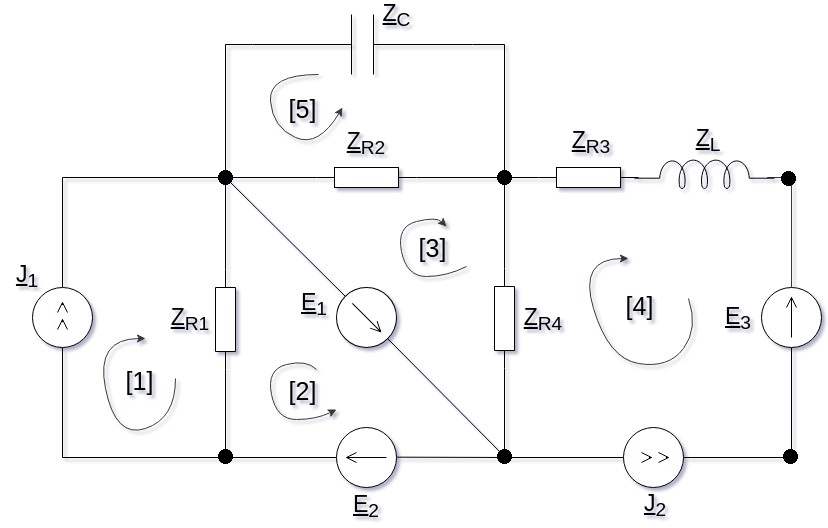
\includegraphics[width=13cm, height=8cm]{bucle.jpg} %\\[0.7cm]
	\end{center}

	 \begin{large} \[ \left\{ \begin{array}{ll}
		$[1]: $ \underline{U}_1 + \underline{U}_9 = 0 \\
		$[2]: $ \underline{U}_1 + \underline{U}_6 + \underline{U}_2  = 0 \\
		$[3]: $ \underline{U}_2 + \underline{U}_3 + \underline{U}_7 = 0 \\
		$[4]: $ \underline{U}_4 + \underline{U}_5 - \underline{U}_7 - \underline{U}_8 = 0 \\
		$[5]: $ \underline{U}_3 - \underline{U}_{10} = 0 \\
	\end{array} \right. \] \end{large}

	Proced\u am la fel ca mai sus \c si ne rezult\u a sistemul:

	 \begin{large} \[ \left\{ \begin{array}{ll}
		\underline{Z}_{R_1} \cdot \underline{I}_5 + \underline{U}_9 = 0 \\
		\underline{Z}_{R_1} \cdot \underline{I}_5 = - \underline{E}_1 - \underline{E}_2 \\
		\underline{Z}_{R_2} \cdot \underline{I}_8 + \underline{Z}_{R_4} \cdot \underline{I}_3 =  - \underline{E}_1 \\
		(\underline{Z}_{R_3} + \underline{Z}_L) \cdot \underline{I}_9 + \underline{U}_5 - \underline{Z}_{R_4} \cdot \underline{I}_3 = \underline{E}_3 \\
		\underline{Z}_{R_2} \cdot \underline{I}_{8} - \underline{Z}_C \cdot \underline{I}_{10} = 0;  \par
	\end{array} \right. \] \end{large}

	Reunind cele dou\u a sisteme, ob\c tinem un sistem de 11 ecua\c tii liniare complexe, cu 11 necunoscute, deci matricea coeficien\c tilor \textbf{A} va fi de $ 11 \times 11 $, iar \textbf{b}, un vector coloan\u a, reprezent\^ and coloana termenilor liberi, va avea tot 11 elemente. Astfel, putem scrie sistemul de ecua\c tii liniare sub forma matriceal\u a \textbf{Ax = b}, unde \textbf{x} este vectorul solu\c tie $ ( [\underline{I}_2, \underline{I}_3, \underline{I}_4, \underline{I}_5, \underline{I}_6, \underline{I}_7, \underline{I}_8, \underline{I}_9, \underline{I}_{10}, \underline{U}_5, \underline{U}_9] ) $, apoi s\u a-l rezolv\u am cu ajutorul unui utilitar numeric precum GNU Octave \cite{label2}.
	
	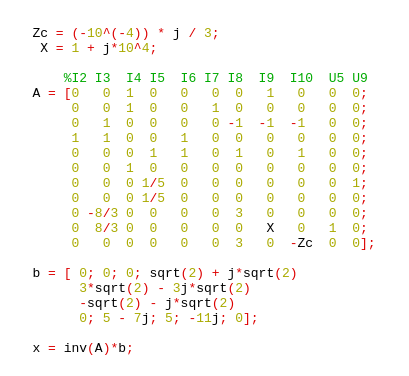
\includegraphics[width=14cm, height=12cm]{octave1.png}

	Cea mai simpl\u a, dar, totodat\u a, ineficient\u a metod\u a de rezolvare a sistemului este s\u a \^ inmul\c tim ecua\c tia matriceal\u a \^ in partea st\^ ang\u a cu \textbf{A$^{-1}, $} rezult\^ and solu\c tia \textbf{x = A$^{-1} $ b}.

	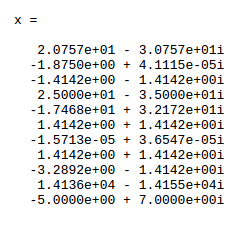
\includegraphics[width=6.5cm, height=6.5cm]{octave2.png}


\end{itemize} \par

\end{subsection}

% -------------------------------------------------------------------------- c) ----------------------------------------------------------------------------------

\begin{subsection}{Bilan\c tul puterilor complexe \\}

	Calcul\^ and sumele puterilor debitate pe receptoare \c si pe generatoare, separat, ob\c tinem:
\begin{large}
	$$ \sum_R^{\underline{S}}  = \underline{U}_1 \cdot \underline{I}_5^* + \underline{U}_3 \cdot \underline{I}_8^* + \underline{U}_4 \cdot \underline{I}_9^* + \underline{U}_7 \cdot \underline{I}_3^*  + \underline{U}_{10} \cdot \underline{I}_{10}^* $$
	$$ = \underline{Z}_1 \cdot \underline{I}_5^2 + \underline{Z}_{R_2} \cdot \underline{I}_8^2 + (\underline{Z}_{R_3} + \underline{Z}_L) \cdot \underline{I}_9^2 + \underline{Z}_{R_4} \cdot \underline{I}_3^2 + \underline{Z}_C \cdot \underline{I}_{10}^2 $$

	$$ \sum_G^{\underline{S}}  = \underline{U}_2 \cdot \underline{I}_6^* + \underline{U}_6 \cdot \underline{I}_2^* + \underline{U}_5 \cdot \underline{I}_7^* + \underline{U}_8 \cdot \underline{I}_4^*  + \underline{U}_9 \cdot \underline{I}_1^* $$ 
	$$ = \underline{E}_1 \cdot \underline{I}_6^* + \underline{U}_5 \cdot \underline{J}_2^* - \underline{U}_9 \cdot \underline{J}_1^* + \underline{E}_3 \cdot \underline{I}_4^* - \underline{E}_2 \cdot \underline{I}_2^* $$
\end{large} 

\begin{center}
	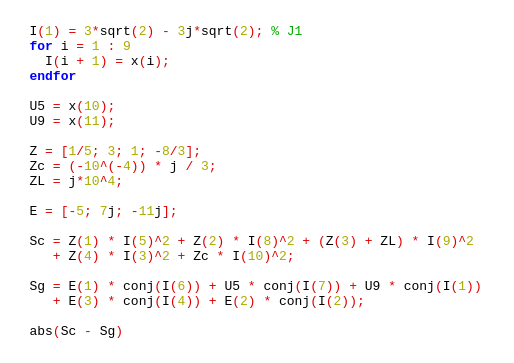
\includegraphics[width=14cm, height=9.5cm]{bilant.png}
	Verificarea bilan\c tului de puteri folosind Octave \\[1.5cm]
\end{center}
\pagebreak
\end{subsection}

% -------------------------------------------------------------------------- d) ----------------------------------------------------------------------------------

\begin{subsection}{Reprezentarea grafic\u a a unei m\u arimi ob\c tinute \\[0.5cm]}
	
	Pentru simplitate, am ales curentul \begin{large} $ \underline{I}_5 = 25 - 35j, $ \end{large} din care ob\c tinem valoarea efectiv\u a \begin{large} $ I_5 = \sqrt{25^2 + 35^ 2} = 43.012 $ \end{large} \c si faza ini\c tial\u a \begin{large} $ \phi_{I_5} = arctg(-\frac{35}{25}) = -0.95055, $ \end{large} deci, forma sinusoidal\u a va fi \begin{large} $ I_5\sqrt2 \cdot sin(\omega t + \phi_{I_5}). $ \end{large} Rezult\u a:
	\begin{large} $$ i_5(t) = 60.828 \cdot sin(100\pi t - 0.95055) $$ \end{large} \\
	
\begin{center}
	\includegraphics[width=10cm, height=2.75cm]{octave3.png}
	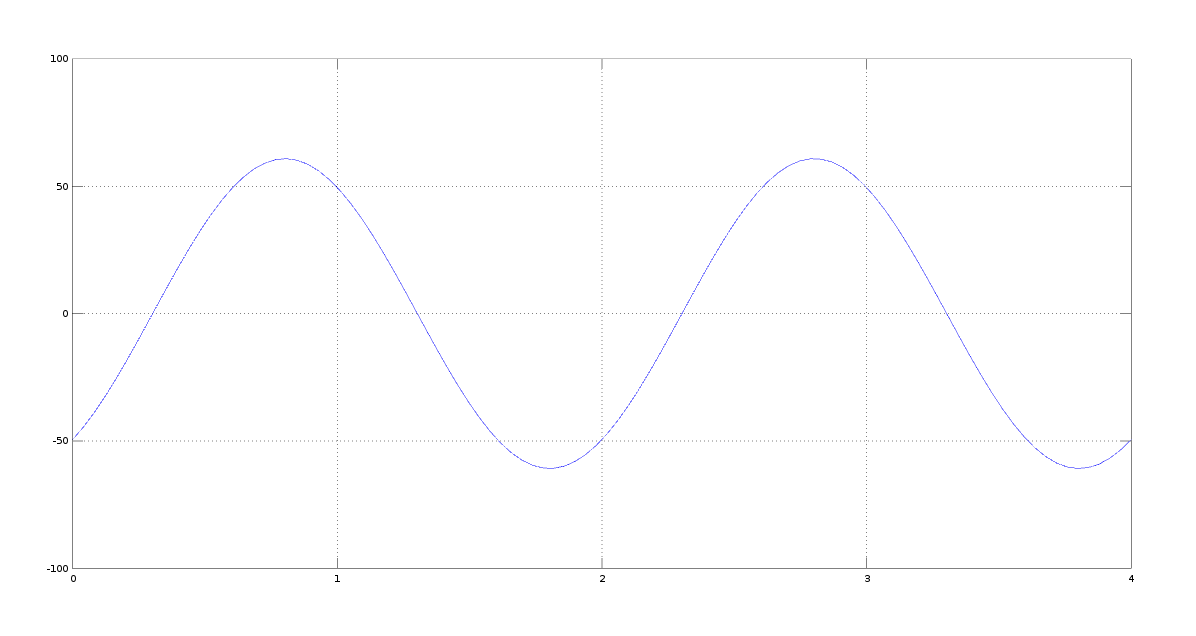
\includegraphics[width=15cm, height=10cm]{grafic.png} \\[1.5cm]
\end{center}

\end{subsection}
\end{section}

% -----------------------------------------------------------------------------------------------------------------------------------------------------------------
% --------------------------------------------------------------------------- 2 ----------------------------------------------------------------------------------

\begin{section}{Rezolvarea circuitelor \^ in regim tranzitoriu \\[0.5cm]}

	Pentru aceast\u a cerin\c t\u a am p\u astrat amplasarea bobinei \c si condensatorului ad\u augate anterior \c si am eliminat latura (1, 5), apoi am trecut toate m\u arimile \^ in opera\c tional. \\

\begin{center}
	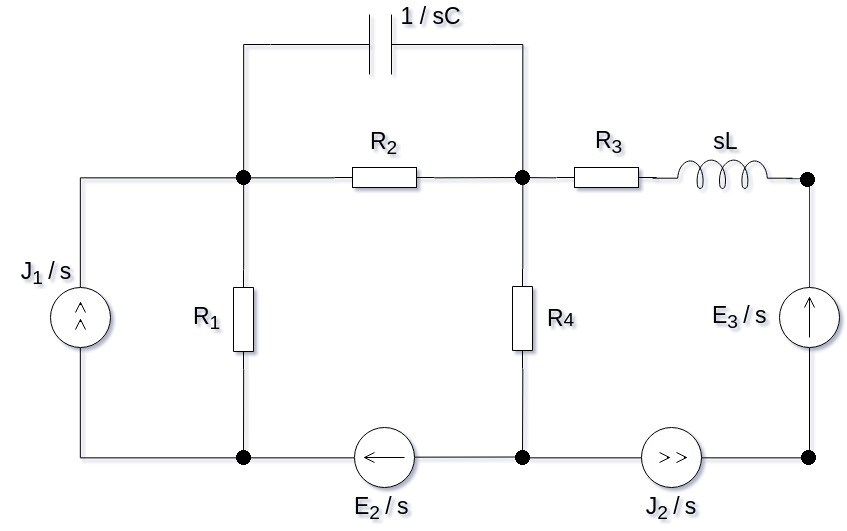
\includegraphics[width=13cm, height=8cm]{operational.jpg} \\
	Noul circuit, trecut \^ in opera\c tional \\[2cm]
	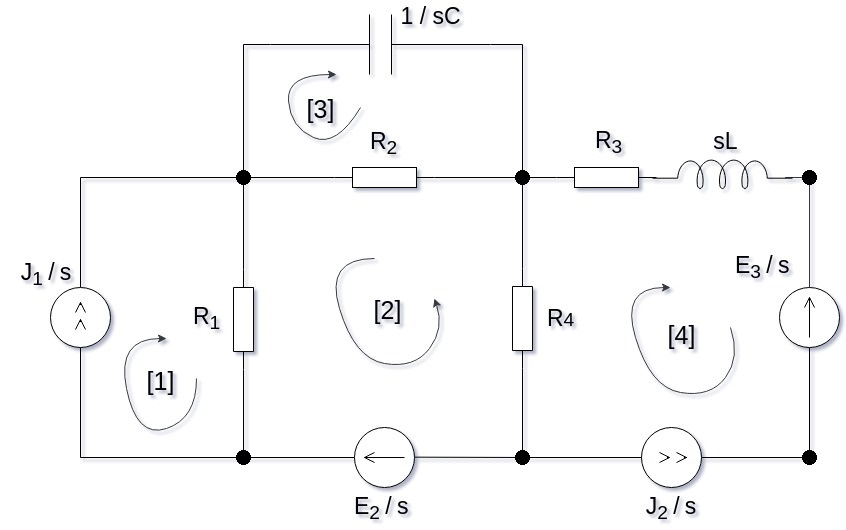
\includegraphics[width=13cm, height=8cm]{opbucle.jpg} \\
	Alegem \c si sensurile de parcurgere pentru bucle \\[1.7cm]
	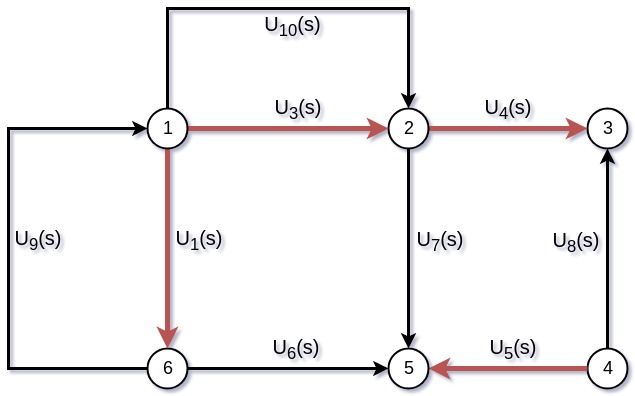
\includegraphics[width=13cm, height=8cm]{grafUop.jpg} \\ 
	Noul graf de tensiuni \\[2cm]
	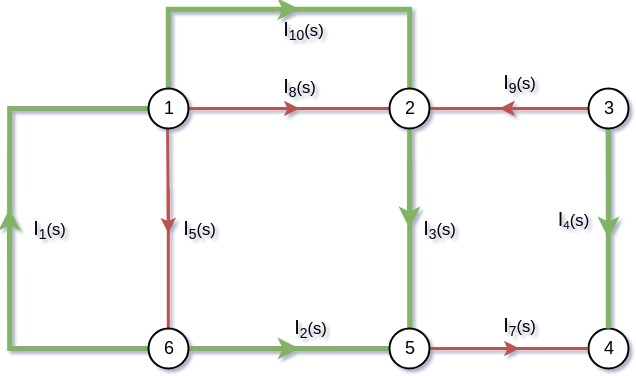
\includegraphics[width=13cm, height=8cm]{grafIop.jpg} \\
	Noul graf de curen\c ti  \\[1cm] 
\end{center}

\begin{itemize}
	\item Din nou, aplic\u am teorema I a lui Kirchhoff pentru $ N - 1 $ noduri:
	
 	\begin{large} \[ \left\{ \begin{array}{ll}
		(1): {I}_1 -  {I}_5 - {I}_8 - {I}_{10} = 0 \\
		(2): {I}_8 + {I}_9  + {I}_{10} - {I}_3 = 0 \\
		(3): {I}_4 + {I}_9 = 0 \\
		(4): {I}_4 + {I}_7 = 0 \\
		(5): {I}_2 + {I}_3 - {I}_7 = 0 \\
	\end{array} \right. \] \end{large}

	\^ Inlocuind cu valorile cunoscute \c si trec\^ and necunoscutele \^ in membrul drept, ob\c tinem sistemul: 

 	\begin{large} \[ \left\{ \begin{array}{ll}
		{I}_5 + {I}_8 + {I}_{10} = \frac{{J}_1}{s} \\
		{I}_3 - {I}_8 - {I}_9 - {I}_{10}  = 0 \\		
		{I}_4 + {I}_9 = 0 \\
		{I}_4 = -\frac{{J}_2}{s}\\		
		{I}_2 + {I}_3 =  \frac{{J}_2}{s} \\
	\end{array} \right. \] \end{large}

	\item Aplic\u am teorema a II-a a lui Kirchhoff pe $ B $ bucle:

	 \begin{large} \[ \left\{ \begin{array}{ll}
		$[1]: $ {U}_1 + {U}_9 = 0 \\
		$[2]: $ {U}_1 + {U}_6 - {U}_3 - U_7  = 0 \\
		$[3]: $ {U}_3 - {U}_{10} = 0 \\
		$[4]: $ {U}_4 + {U}_5 - {U}_7 - {U}_8 = 0 \\
	\end{array} \right. \] \end{large}

	Proced\u am la fel ca mai sus \c si ne rezult\u a sistemul:

	 \begin{large} \[ \left\{ \begin{array}{ll}
		{R_1} \cdot {I}_5 + {U}_9 = 0 \\
		{R_1} \cdot {I}_5 - {R_2} \cdot {I}_8 - {R_4} \cdot {I}_3 = -\frac{E_2}{s} \\
		{R_2} \cdot {I}_8 - \frac{1}{sC} \cdot {I}_{10} =  0 \\
		({R_3} + sL) \cdot {I}_9 + {U}_5 - {R_4} \cdot \underline{I}_3 = \frac{E_3}{s} \\ \par
	\end{array} \right. \] \end{large}
	
\begin{center}
	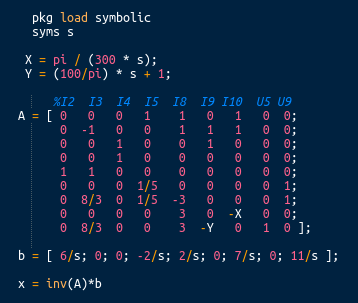
\includegraphics[width=12cm, height=10cm]{symb.png}
\end{center}
\end{itemize}
\end{section}
\pagebreak

%----------------------------------------------------------------------------------------------------------------------------------------------------------------
% --------------------------------------------------------------------------- 3 ----------------------------------------------------------------------------------

\begin{section}{Calculul \c si reprezentarea unui c\^ amp electric \\}

	O distribu\c tie foarte simpl\u a de sarcin\u a care s\u a depind\u a numai de raz\u a \^ intr-un sistem de coordonate sferice este: \\

\begin{center} \begin{large}
	$ \rho(r, \theta, \phi) = 
		\begin{cases} r, 
			$ dac\u a $ r \in [0, a] \\
			0, $ \^ in rest $
		\end{cases} $
\end{large} \end{center}

	Conform legii fluxului electric: 
	\begin{large}
	$$ \Psi_\Sigma = q_{D_\Sigma} $$
	$$ \Longleftrightarrow  \int_\Sigma{\overline{D} \cdot dA} = \int_{D_\Sigma}{\rho \cdot dV} $$
	$$ \Longrightarrow  4\pi r^2 \cdot \overline{D} = \Psi $$
	$$ \Longleftrightarrow   \overline{D} = \frac{\Psi}{4\pi r^2} $$
	\end{large}	

	Cum 	\begin{large} $ \Psi_\Sigma = \int_{D_\Sigma}{\rho \cdot dV}, $ \end{large} \^ in coordonate sferice, \begin{large} $ \theta $ \end{large} \c si \begin{large} $ \phi \in [0, 2\pi], $ \end{large} iar raza \begin{large} $ r \in [0, a], $ \end{large} deci pe intervalul $ [0, a] $ vom avea:
	\begin{large}
	$$ \Psi = \int_{0}^{2\pi}{ \int_{0}^{2\pi}{ \int_{0}^{a}{\rho \cdot dr \cdot d\theta \cdot d\phi}}} = \int_{0}^{2\pi}{ \int_{0}^{2\pi}{ \int_{0}^{a}{r \cdot dr \cdot d\theta \cdot d\phi}}} $$
	$$= \int_{0}^{2\pi}{d\phi} \cdot \int_{0}^{2\pi}{d\theta} \cdot \int_{0}^{a}{r \cdot dr} = 2 \pi^2 a^2. $$
	\end{large}
	\begin{large} $$ \Longrightarrow   \overline{D} = \frac{2 \pi^2 a^2}{4\pi r^2} = \frac{\pi a^2}{2r^2}. $$ \end{large}  \\ \par
	Pentru orice alt\u a valoare a lui $ r, $ $ \rho $ va fi 0, integrala va fi 0, deci \c si $ \overline{D} $ va fi tot 0. 
\pagebreak
\begin{center}
	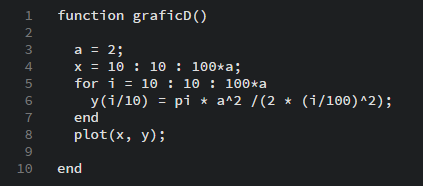
\includegraphics[width=11cm, height=6cm]{graficD.png}
	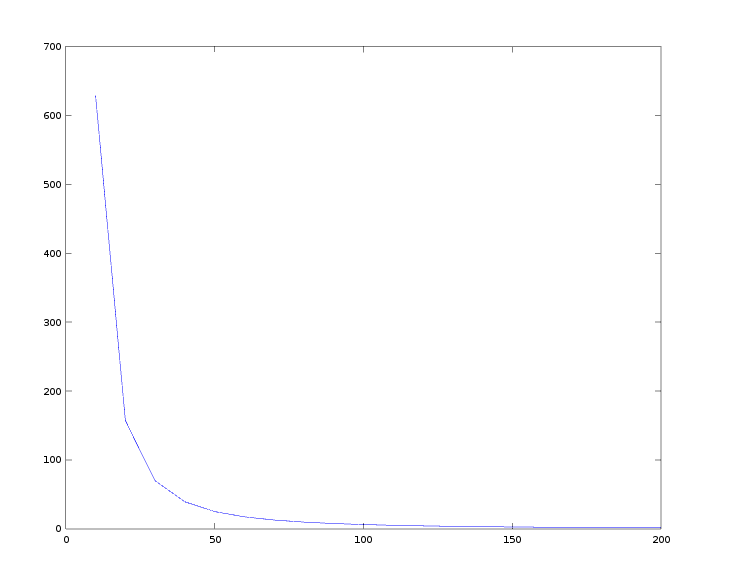
\includegraphics[width=14cm, height=14cm]{graficsD.png}
\end{center}

\end{section}

% -----------------------------------------------------------------------------------------------------------------------------------------------------------------

\end{document}